\documentclass[12pt,a4paper]{article}

% Packages
\usepackage[utf8]{inputenc}
\usepackage[T1]{fontenc}
\usepackage{geometry}
\usepackage{graphicx}
\usepackage{xcolor}
\usepackage{listings}
\usepackage{booktabs}
\usepackage{array}
\usepackage{tikz}
\usepackage{fancybox}
\usepackage{tcolorbox}
\usepackage{enumitem}
\usepackage{hyperref}
\usepackage{fancyhdr}
\usepackage{titlesec}

% Page geometry
\geometry{margin=2.5cm}

% Colors
\definecolor{mastercolor}{RGB}{70, 130, 180}
\definecolor{slavecolor}{RGB}{60, 179, 113}
\definecolor{hdfscolor}{RGB}{255, 165, 0}
\definecolor{codebackground}{RGB}{245, 245, 245}
\definecolor{boxcolor}{RGB}{230, 240, 250}

% TikZ libraries
\usetikzlibrary{shapes.geometric, arrows, positioning, fit, backgrounds, calc}

% Code listing style
\lstset{
    backgroundcolor=\color{codebackground},
    basicstyle=\ttfamily\small,
    breaklines=true,
    frame=single,
    framerule=0pt,
    xleftmargin=10pt,
    xrightmargin=10pt,
    showstringspaces=false
}

% Custom tcolorbox styles
\tcbuselibrary{skins, breakable}

\newtcolorbox{infobox}[1][]{
    colback=boxcolor,
    colframe=mastercolor,
    fonttitle=\bfseries,
    title=#1,
    breakable
}

\newtcolorbox{warningbox}[1][]{
    colback=yellow!10,
    colframe=orange!80!black,
    fonttitle=\bfseries,
    title=#1,
    breakable
}

% Title formatting
\titleformat{\section}{\Large\bfseries\color{mastercolor}}{\thesection}{1em}{}
\titleformat{\subsection}{\large\bfseries\color{mastercolor!80!black}}{\thesubsection}{1em}{}

% Document info
\title{\Huge\textbf{Hadoop Infrastructure Explained}\\[0.5cm]
\Large With a Practical Sales Example}
\author{Big Data - LAB1 Hadoop}
\date{\today}

\begin{document}

\maketitle
\tableofcontents
\newpage

%==============================================================================
\section{Hadoop Infrastructure Explained with Your Sales Example}
%==============================================================================

This document explains each component of Hadoop and its role in processing sales data using MapReduce.

%==============================================================================
\section{Your Setup}
%==============================================================================

\begin{center}
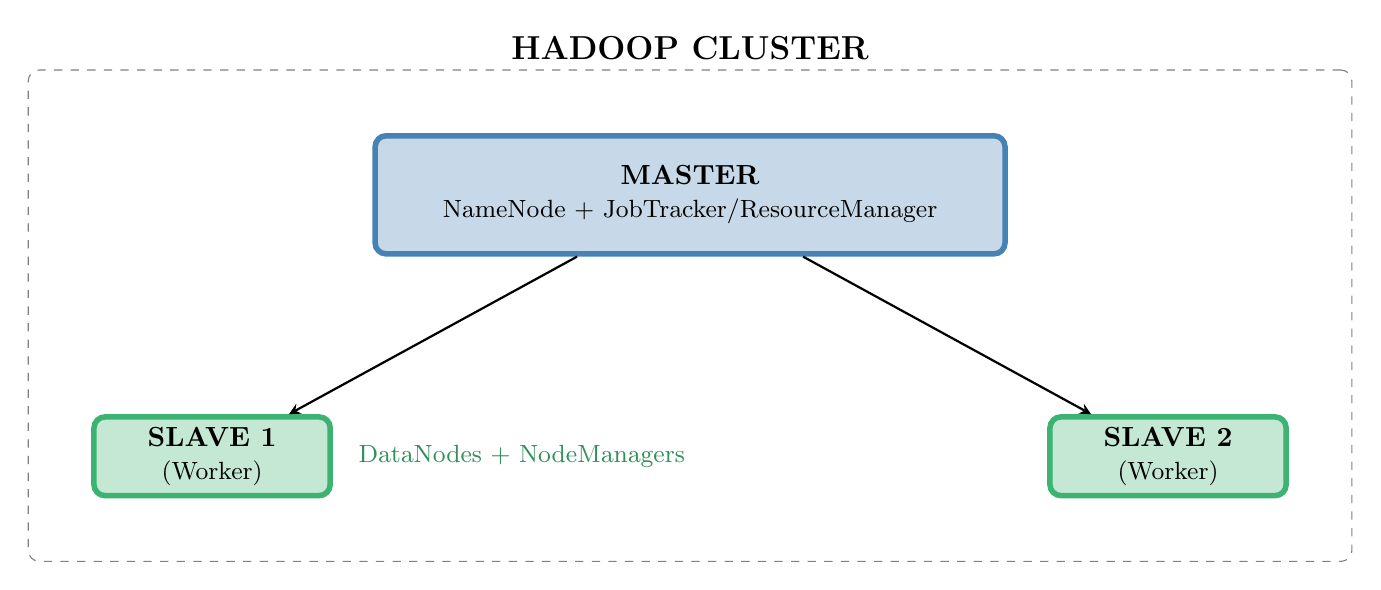
\begin{tikzpicture}[
    node distance=1.5cm,
    box/.style={rectangle, draw, rounded corners, minimum width=3cm, minimum height=1cm, align=center},
    masterbox/.style={box, fill=mastercolor!30, draw=mastercolor, line width=2pt},
    slavebox/.style={box, fill=slavecolor!30, draw=slavecolor, line width=2pt},
    arrow/.style={->, thick, >=stealth}
]
    % Master node
    \node[masterbox, minimum width=8cm, minimum height=1.5cm] (master) {
        \textbf{MASTER}\\
        {\small NameNode + JobTracker/ResourceManager}
    };
    
    % Slave nodes
    \node[slavebox, below left=2cm and 0.5cm of master] (slave1) {
        \textbf{SLAVE 1}\\
        {\small (Worker)}
    };
    
    \node[slavebox, below right=2cm and 0.5cm of master] (slave2) {
        \textbf{SLAVE 2}\\
        {\small (Worker)}
    };
    
    % Arrows
    \draw[arrow] (master) -- (slave1);
    \draw[arrow] (master) -- (slave2);
    
    % Labels
    \node[right=0.2cm of slave1, slavecolor!80!black] {\small DataNodes + NodeManagers};
    
    % Cluster box
    \begin{scope}[on background layer]
        \node[draw=gray, dashed, rounded corners, fit=(master)(slave1)(slave2), 
              inner sep=0.8cm, label={[font=\large\bfseries]above:HADOOP CLUSTER}] {};
    \end{scope}
\end{tikzpicture}
\end{center}

%==============================================================================
\section{HDFS (Hadoop Distributed File System)}
%==============================================================================

\begin{infobox}[What is HDFS?]
A file system that stores data \textbf{across multiple machines}.
\end{infobox}

\subsection{In Your Example}

When you upload \texttt{Command-sales.txt} to HDFS, here's what happens:

\begin{center}
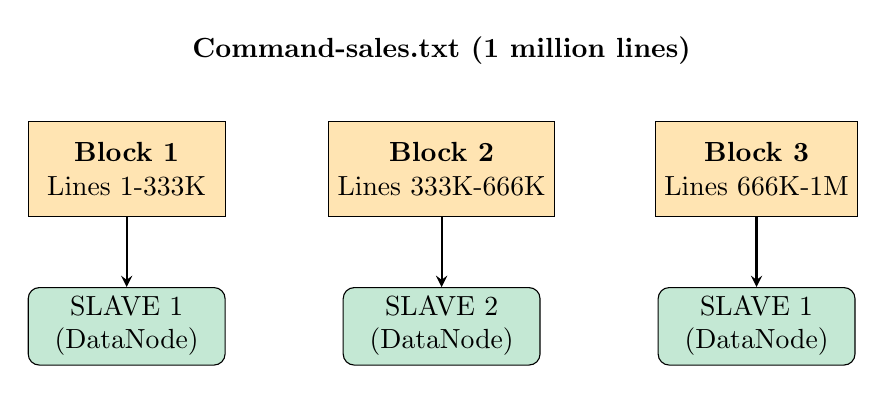
\begin{tikzpicture}[
    block/.style={rectangle, draw, fill=hdfscolor!30, minimum width=2.5cm, minimum height=1.2cm, align=center},
    slave/.style={rectangle, draw, fill=slavecolor!30, rounded corners, minimum width=2.5cm, minimum height=0.8cm, align=center},
    arrow/.style={->, thick, >=stealth}
]
    % File label
    \node[font=\bfseries] at (0, 3) {Command-sales.txt (1 million lines)};
    
    % Blocks
    \node[block] (b1) at (-4, 1.5) {\textbf{Block 1}\\Lines 1-333K};
    \node[block] (b2) at (0, 1.5) {\textbf{Block 2}\\Lines 333K-666K};
    \node[block] (b3) at (4, 1.5) {\textbf{Block 3}\\Lines 666K-1M};
    
    % Slaves
    \node[slave] (s1) at (-4, -0.5) {SLAVE 1\\(DataNode)};
    \node[slave] (s2) at (0, -0.5) {SLAVE 2\\(DataNode)};
    \node[slave] (s3) at (4, -0.5) {SLAVE 1\\(DataNode)};
    
    % Arrows
    \draw[arrow] (b1) -- (s1);
    \draw[arrow] (b2) -- (s2);
    \draw[arrow] (b3) -- (s3);
\end{tikzpicture}
\end{center}

\begin{warningbox}[Key Point]
\textbf{HDFS splits your file into blocks (default 128MB) and distributes them!}
\end{warningbox}

%==============================================================================
\section{NameNode (Lives on Master)}
%==============================================================================

\begin{table}[h]
\centering
\renewcommand{\arraystretch}{1.4}
\begin{tabular}{>{\bfseries}l p{10cm}}
\toprule
Aspect & Description \\
\midrule
What is it? & The ``brain'' of HDFS - stores \textbf{metadata only} \\
What it stores & File names, directory structure, which block is on which DataNode \\
Does NOT store & The actual data! \\
\bottomrule
\end{tabular}
\end{table}

\subsection{In Your Example}

\begin{tcolorbox}[colback=codebackground, colframe=gray, title=NameNode's Memory]
\begin{verbatim}
File: /user/hadoop/sales/Command-sales.txt
  - Block 1 → Slave1, Slave2 (replicated)
  - Block 2 → Slave2, Slave1 (replicated)
  - Block 3 → Slave1, Slave2 (replicated)
\end{verbatim}
\end{tcolorbox}

\begin{infobox}[Analogy]
\textbf{It's like a phonebook:} It knows WHERE everything is, but doesn't have the data itself.
\end{infobox}

%==============================================================================
\section{DataNode (Lives on Slaves/Workers)}
%==============================================================================

\begin{table}[h]
\centering
\renewcommand{\arraystretch}{1.4}
\begin{tabular}{>{\bfseries}l p{10cm}}
\toprule
Aspect & Description \\
\midrule
What is it? & The ``muscles'' - stores \textbf{actual data blocks} \\
What it does & Stores blocks, sends data when requested, reports health to NameNode \\
\bottomrule
\end{tabular}
\end{table}

\subsection{In Your Example}

\begin{center}
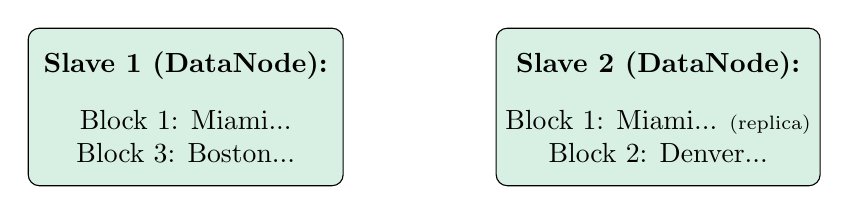
\begin{tikzpicture}[
    slavebox/.style={rectangle, draw, fill=slavecolor!20, rounded corners, minimum width=4cm, minimum height=2cm, align=center}
]
    \node[slavebox] (s1) at (-3, 0) {
        \textbf{Slave 1 (DataNode):}\\[0.3cm]
        Block 1: Miami...\\
        Block 3: Boston...
    };
    
    \node[slavebox] (s2) at (3, 0) {
        \textbf{Slave 2 (DataNode):}\\[0.3cm]
        Block 1: Miami... {\scriptsize (replica)}\\
        Block 2: Denver...
    };
\end{tikzpicture}
\end{center}

%==============================================================================
\section{Secondary NameNode}
%==============================================================================

\begin{table}[h]
\centering
\renewcommand{\arraystretch}{1.4}
\begin{tabular}{>{\bfseries}l p{10cm}}
\toprule
Aspect & Description \\
\midrule
What is it? & A \textbf{helper} for the NameNode (NOT a backup!) \\
What it does & Periodically merges edit logs with the filesystem image \\
Purpose & Reduces NameNode restart time \\
\bottomrule
\end{tabular}
\end{table}

\subsection{In Your Example}

\begin{center}
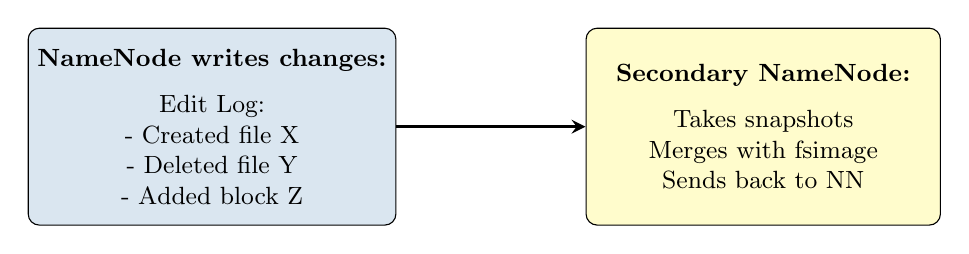
\begin{tikzpicture}[
    box/.style={rectangle, draw, rounded corners, minimum width=4.5cm, minimum height=2.5cm, align=center, font=\small},
    arrow/.style={->, thick, >=stealth}
]
    \node[box, fill=mastercolor!20] (nn) at (-3.5, 0) {
        \textbf{NameNode writes changes:}\\[0.2cm]
        Edit Log:\\
        - Created file X\\
        - Deleted file Y\\
        - Added block Z
    };
    
    \node[box, fill=yellow!20] (snn) at (3.5, 0) {
        \textbf{Secondary NameNode:}\\[0.2cm]
        Takes snapshots\\
        Merges with fsimage\\
        Sends back to NN
    };
    
    \draw[arrow, very thick] (nn) -- (snn);
\end{tikzpicture}
\end{center}

\begin{warningbox}[Common Misconception]
The Secondary NameNode is \textbf{NOT} a failover for NameNode!
\end{warningbox}

%==============================================================================
\section{Master vs NameNode / Slaves vs DataNodes}
%==============================================================================

\subsection{Are they the same?}

\textbf{Not exactly!} The Master and Slaves are \textbf{machines}, while NameNode/DataNode are \textbf{processes}:

\begin{table}[h]
\centering
\renewcommand{\arraystretch}{1.5}
\begin{tabular}{>{\bfseries}l p{9cm}}
\toprule
Machine & Processes Running \\
\midrule
Master & NameNode + ResourceManager (YARN) + Secondary NameNode \\
Slave 1 & DataNode + NodeManager \\
Slave 2 & DataNode + NodeManager \\
\bottomrule
\end{tabular}
\end{table}

\subsection{Visual Representation}

\begin{center}
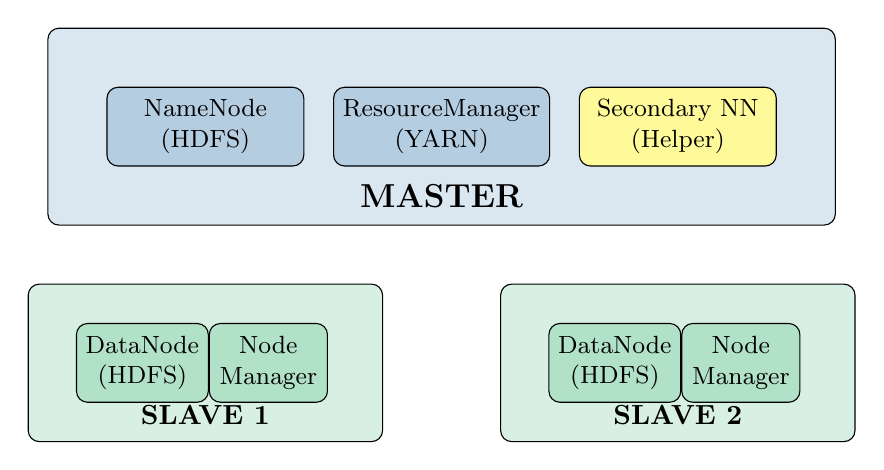
\begin{tikzpicture}[
    machine/.style={rectangle, draw, rounded corners, minimum width=10cm, minimum height=2cm, align=center},
    process/.style={rectangle, draw, fill=white, rounded corners, minimum width=2.5cm, minimum height=1cm, align=center, font=\small},
    slavemachine/.style={rectangle, draw, rounded corners, minimum width=4.5cm, minimum height=2cm, align=center}
]
    % Master
    \node[machine, fill=mastercolor!20, minimum height=2.5cm] (master) at (0, 3) {};
    \node[above=0.1cm of master.south, font=\bfseries\large] {MASTER};
    
    \node[process, fill=mastercolor!40] at (-3, 3) {NameNode\\(HDFS)};
    \node[process, fill=mastercolor!40] at (0, 3) {ResourceManager\\(YARN)};
    \node[process, fill=yellow!40] at (3, 3) {Secondary NN\\(Helper)};
    
    % Slaves
    \node[slavemachine, fill=slavecolor!20] (slave1) at (-3, 0) {};
    \node[above=0.1cm of slave1.south, font=\bfseries] {SLAVE 1};
    \node[process, fill=slavecolor!40, minimum width=1.5cm] at (-3.8, 0) {DataNode\\(HDFS)};
    \node[process, fill=slavecolor!40, minimum width=1.5cm] at (-2.2, 0) {Node\\Manager};
    
    \node[slavemachine, fill=slavecolor!20] (slave2) at (3, 0) {};
    \node[above=0.1cm of slave2.south, font=\bfseries] {SLAVE 2};
    \node[process, fill=slavecolor!40, minimum width=1.5cm] at (2.2, 0) {DataNode\\(HDFS)};
    \node[process, fill=slavecolor!40, minimum width=1.5cm] at (3.8, 0) {Node\\Manager};
\end{tikzpicture}
\end{center}

%==============================================================================
\section{How Your MapReduce Job Runs}
%==============================================================================

\subsection{Step-by-Step with Your Sales Example}

\begin{tcolorbox}[colback=codebackground, colframe=gray, title=Command to Run]
\begin{verbatim}
hadoop jar hadoop-streaming.jar \
    -mapper mapper.py \
    -reducer reducer.py \
    -input /sales \
    -output /result
\end{verbatim}
\end{tcolorbox}

%--- STEP 1 ---
\begin{tcolorbox}[colback=mastercolor!10, colframe=mastercolor, title=\textbf{STEP 1: ResourceManager (Master) receives job}]
ResourceManager receives the job request:\\
\textit{``I need to process /sales/Command-sales.txt''}
\end{tcolorbox}

%--- STEP 2 ---
\begin{tcolorbox}[colback=mastercolor!10, colframe=mastercolor, title=\textbf{STEP 2: NameNode provides block locations}]
NameNode says:\\
\textit{``File has 2 blocks: Block1 $\rightarrow$ Slave1, Block2 $\rightarrow$ Slave2''}
\end{tcolorbox}

%--- STEP 3 ---
\begin{tcolorbox}[colback=slavecolor!10, colframe=slavecolor, title=\textbf{STEP 3: ResourceManager launches Mappers WHERE DATA IS}]
\begin{itemize}[noitemsep]
    \item Slave 1: Run \texttt{mapper.py} on Block 1
    \item Slave 2: Run \texttt{mapper.py} on Block 2
\end{itemize}
\vspace{0.3cm}
\textbf{(Data locality! Don't move data, move code!)}
\end{tcolorbox}

%--- STEP 4 ---
\begin{tcolorbox}[colback=hdfscolor!10, colframe=hdfscolor!80!black, title=\textbf{STEP 4: Mappers output (Store, Cost) pairs}]
\begin{center}
\begin{tabular}{ll}
\textbf{Slave 1 outputs:} & \textbf{Slave 2 outputs:} \\
\midrule
Miami \quad 999.99 & Boston \quad 79.99 \\
Denver \quad 150.00 & Miami \quad 29.99 \\
\end{tabular}
\end{center}
\end{tcolorbox}

%--- STEP 5 ---
\begin{tcolorbox}[colback=purple!10, colframe=purple!80!black, title=\textbf{STEP 5: SHUFFLE \& SORT (Hadoop magic!)}]
Group all same keys together, sort alphabetically:
\begin{verbatim}
Boston:  79.99
Denver:  150.00
Miami:   999.99, 29.99
\end{verbatim}
\end{tcolorbox}

%--- STEP 6 ---
\begin{tcolorbox}[colback=red!10, colframe=red!80!black, title=\textbf{STEP 6: Reducer runs (on one or more nodes)}]
\texttt{reducer.py} processes sorted stream:
\begin{itemize}[noitemsep]
    \item $\rightarrow$ Boston \quad 79.99 \quad $\rightarrow$ print ``Boston \quad 79.99''
    \item $\rightarrow$ Denver \quad 150.00 \quad $\rightarrow$ print ``Denver \quad 150.00''
    \item $\rightarrow$ Miami \quad 999.99 $\}$
    \item $\rightarrow$ Miami \quad 29.99 \quad $\}$ $\rightarrow$ print ``Miami \quad 1029.98''
\end{itemize}
\end{tcolorbox}

%--- STEP 7 ---
\begin{tcolorbox}[colback=green!10, colframe=green!60!black, title=\textbf{STEP 7: Output written to HDFS: /result/part-00000}]
\begin{verbatim}
Boston   79.99
Denver   150.00
Miami    1029.98
\end{verbatim}
\end{tcolorbox}

%==============================================================================
\section{Summary Table}
%==============================================================================

\begin{table}[h]
\centering
\renewcommand{\arraystretch}{1.5}
\begin{tabular}{>{\bfseries}l l p{7cm}}
\toprule
Component & Location & Role in Your Example \\
\midrule
HDFS & Across all nodes & Stores \texttt{Command-sales.txt} split into blocks \\
NameNode & Master & Knows which blocks are on which slave \\
DataNode & Slaves 1 \& 2 & Actually stores the data blocks \\
Secondary NameNode & Master (or separate) & Helps NameNode with checkpoints \\
ResourceManager & Master & Schedules where mappers/reducers run \\
NodeManager & Slaves 1 \& 2 & Runs \texttt{mapper.py} and \texttt{reducer.py} \\
\bottomrule
\end{tabular}
\end{table}

%==============================================================================
\section{Key Insight: Data Locality}
%==============================================================================

\begin{center}
\begin{tcolorbox}[colback=yellow!20, colframe=orange, width=12cm, boxrule=2pt]
\begin{center}
\Large\bfseries
``Move computation to data, not data to computation''
\end{center}
\end{tcolorbox}
\end{center}

\vspace{0.5cm}

\begin{table}[h]
\centering
\renewcommand{\arraystretch}{1.5}
\begin{tabular}{cl}
\toprule
& \textbf{Approach} \\
\midrule
\textcolor{red}{\ding{55}} & Copy all data to one machine $\rightarrow$ Process $\rightarrow$ \textbf{Slow!} \\
\textcolor{green}{\ding{51}} & Send \texttt{mapper.py} (tiny file) to where data already is $\rightarrow$ \textbf{Fast!} \\
\bottomrule
\end{tabular}
\end{table}

\vspace{1cm}

\begin{center}
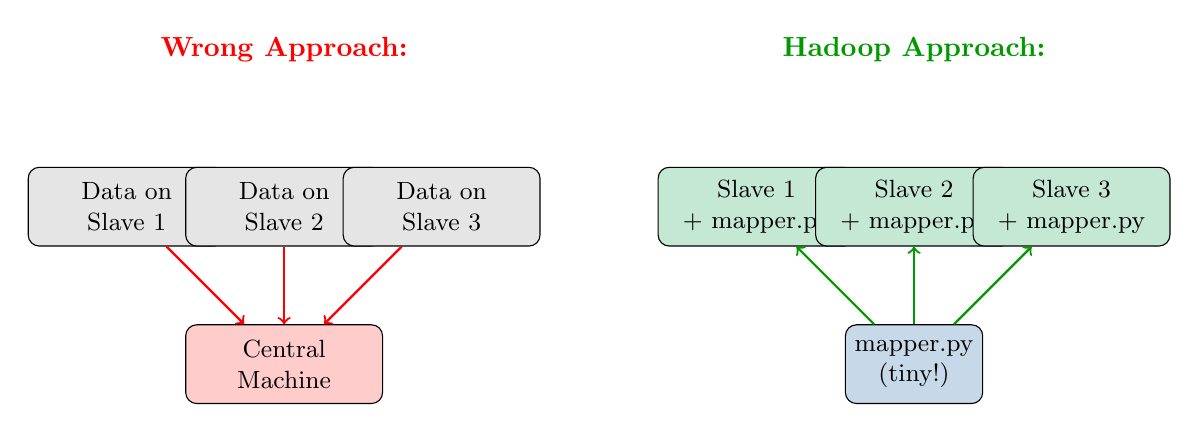
\begin{tikzpicture}[
    node distance=2cm,
    box/.style={rectangle, draw, rounded corners, minimum width=2.5cm, minimum height=1cm, align=center, font=\small}
]
    % Wrong approach
    \node[font=\bfseries\color{red}] at (-4, 2) {Wrong Approach:};
    \node[box, fill=gray!20] (data1) at (-6, 0) {Data on\\Slave 1};
    \node[box, fill=gray!20] (data2) at (-4, 0) {Data on\\Slave 2};
    \node[box, fill=gray!20] (data3) at (-2, 0) {Data on\\Slave 3};
    \node[box, fill=red!20] (central) at (-4, -2) {Central\\Machine};
    
    \draw[->, thick, red] (data1) -- (central);
    \draw[->, thick, red] (data2) -- (central);
    \draw[->, thick, red] (data3) -- (central);
    
    % Right approach
    \node[font=\bfseries\color{green!60!black}] at (4, 2) {Hadoop Approach:};
    \node[box, fill=slavecolor!30] (s1) at (2, 0) {Slave 1\\+ mapper.py};
    \node[box, fill=slavecolor!30] (s2) at (4, 0) {Slave 2\\+ mapper.py};
    \node[box, fill=slavecolor!30] (s3) at (6, 0) {Slave 3\\+ mapper.py};
    
    \node[box, fill=mastercolor!30, minimum width=1.5cm] (code) at (4, -2) {mapper.py\\(tiny!)};
    
    \draw[->, thick, green!60!black] (code) -- (s1);
    \draw[->, thick, green!60!black] (code) -- (s2);
    \draw[->, thick, green!60!black] (code) -- (s3);
\end{tikzpicture}
\end{center}

\end{document}
